% coding:utf-8

%----------------------------------------
%FOSAMATH, a LaTeX-Code for a mathematical summary for basic analysis
%Copyright (C) 2013, Daniel Winz, Ervin Mazlagic, Adrian Imboden, Philipp Langer

%This program is free software; you can redistribute it and/or
%modify it under the terms of the GNU General Public License
%as published by the Free Software Foundation; either version 2
%of the License, or (at your option) any later version.

%This program is distributed in the hope that it will be useful,
%but WITHOUT ANY WARRANTY; without even the implied warranty of
%MERCHANTABILITY or FITNESS FOR A PARTICULAR PURPOSE.  See the
%GNU General Public License for more details.
%----------------------------------------

% coding:utf-8
\section{Definition Differentialgleichungen}
Gleichungen, in der eine Variable, eine von dieser Variable abhängige Funktion 
und Ableitungen beliebigen Grades dieser Funktion vorkommen, werden 
Differentialgleichungen genannt. 
\[ F(x, y, y', y'', \ldots, y^{(n)})=0 \]
$x$ heisst dabei unabhängige und $y$ abhängige Variable. Dafür können auch 
andere Buchstaben als $x$ und $y$ verwendet werden. 
Ableitungen nach t werden auch als $\dot{y}$ geschrieben. 

\section{Gewöhnliche Gleichung $\to$ Differentialgleichung}
Um aus einer gewöhnlichen Gleichung eine Differentialgleichung zu erhalten
kann folgendes Verfahren verwendet werden.
\begin{enumerate}
	\item Anzahl der Parameter ermitteln $\Rightarrow n$
			\[ y = ax \rightarrow n=1 \]
	\item $n$-fach ableiten $\Rightarrow n+1$ Gleichungen
			\[ y' = a  \]
	\item Gleichungssystem lösen
			\[ y=ax \Rightarrow a=\frac{y}{x} \]
	\item erhaltene Parameter einsetzen	
			\[ y'=\frac{y}{x} \]
\end{enumerate}

\section{Grundbegriffe}

\subsection{Ordnung}
Die Ordnung einer Differentialgleichung wird durch die höchste vorkommende 
Ordnung der Ableitungen von $y$ bestimmt. 

\subsection{Grad}
Der Grad einer Differentialgleichung wird durch die höchste vorkommende Potenz 
von $y$ oder den Ableitungen von $y$ bestimmt. Potenzen der unabhängigen 
Variable werden dabei nicht berücksichtigt. 
\subsubsection*{Achtung:}
$y \cdot y' \quad \rightarrow \quad$ Grad 2

\subsubsection{Grad 1}
Differentialgleichungen vom Grad 1 nennt man linear. 

\subsection{Lösungen}
Eine Gleichung der Form
\[ F(x, y, y', y'', \ldots, y^{(n)})=0 \]
besitzt eine allgemeine Lösung. Diese enthält $n$ Parameter ($n$-parametrige 
Kurvenschar). Jede Kombination dieser Parameter ergibt eine spezielle bzw. 
partikuläre Lösung. Durch das Festlegen spezieller Werte für 
$y, y', y'', \ldots, y^{(n)}$ an einer beliebigen Stelle $x_0$ erhält man Werte 
für die $n$ Parameter und somit eine partikuläre Lösung. 

\section{Richtungsfeld und Trajektorien}
Ein Richtungsfeld ist ein Abbild einer Differentialgleichung im Raum.
Dabei wird jedem Punkt im Raum eine Steigung (\emph{Differential})
zugewiesen. Im folgenden ein Beispiel eines solchen Richtungsfeldes.

\begin{figure}[h!]
	\centering
	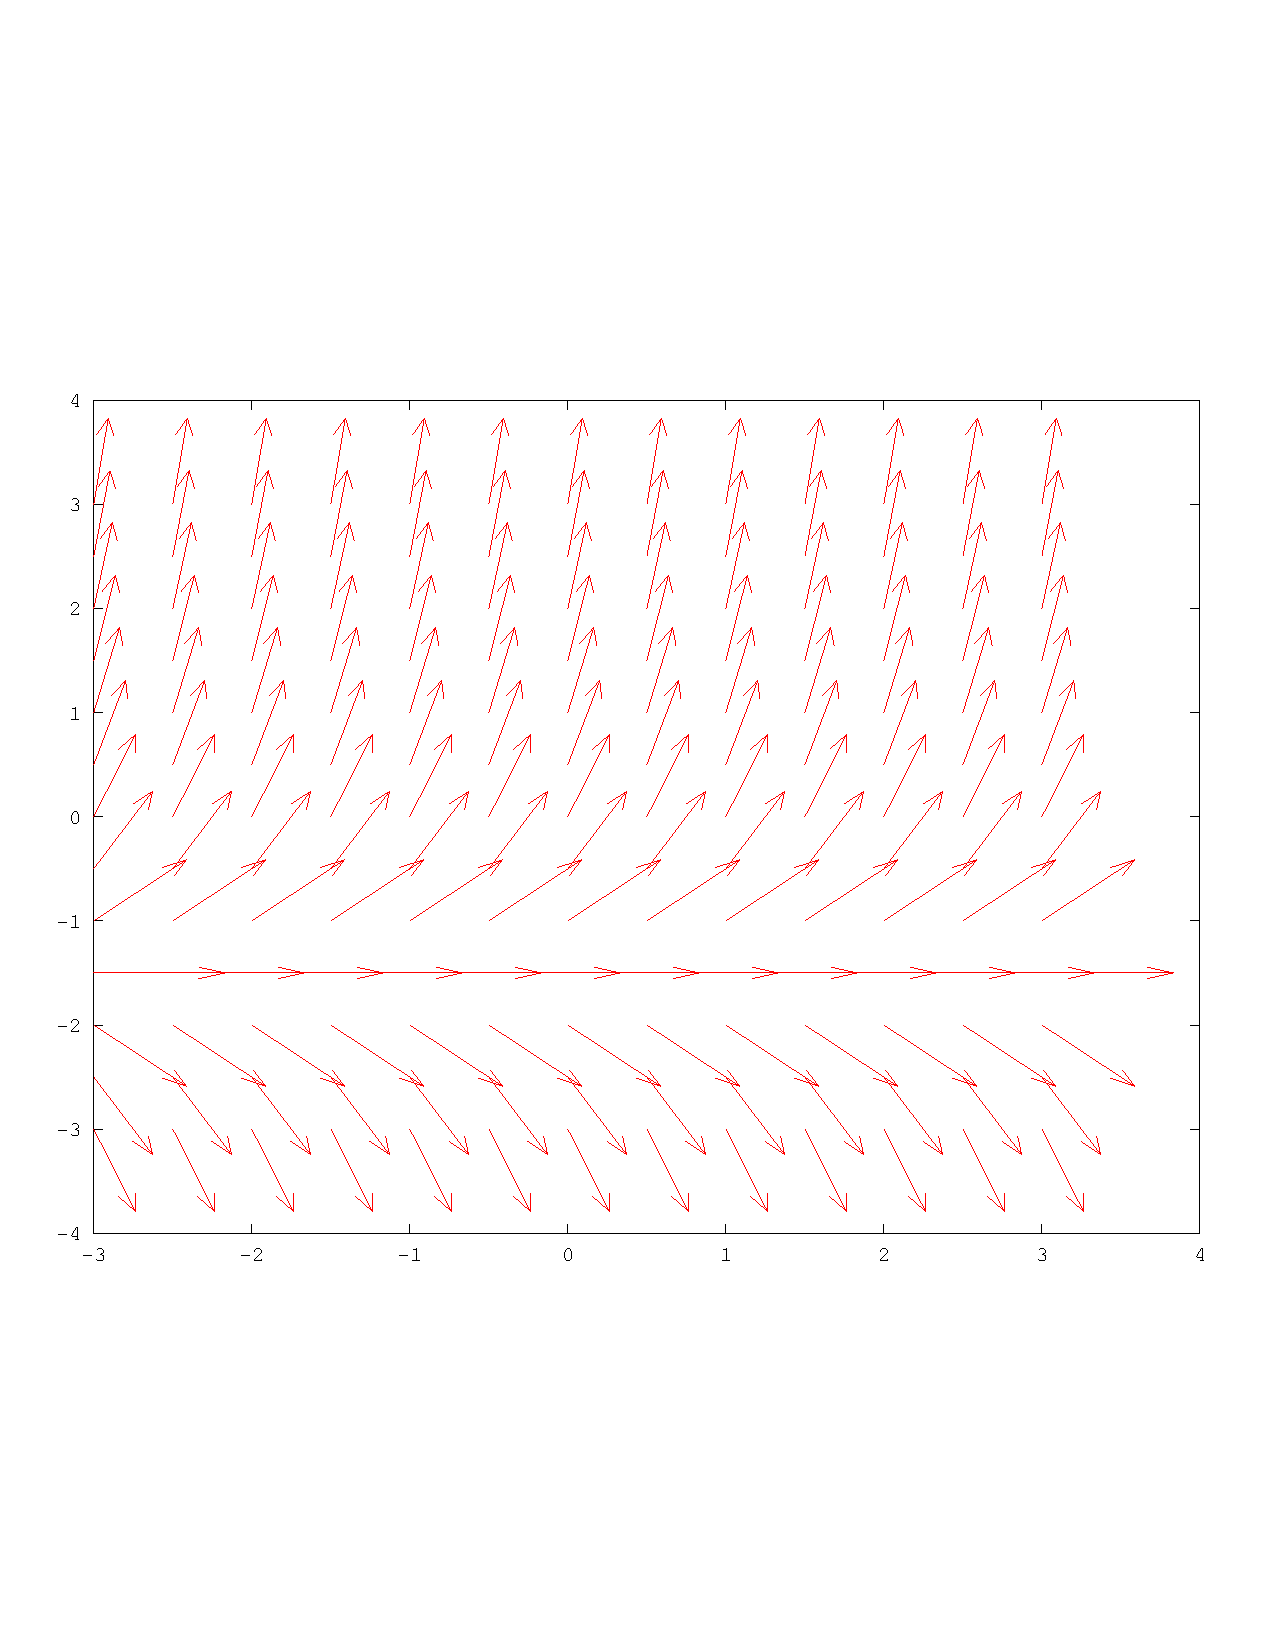
\includegraphics[width=0.8\textwidth]{field.pdf}
	\caption{Richtungsfeld der Differentialgleichung $y'=3+2y$}
\end{figure}

\noindent
Die Berechnung der einzelnen Punkte erfolgt durch reines einsetzen.
Z.B. für den Punkt $P(x=1, y=-1)$ ergibt sich $3+2(-1)=1$ usw.

\subsection{Trajektorien}
Eine Trajektorie ist eine Bahn oder eine Kurve. Sie kann die Lösung einer 
Differentialgleichung darstellen. Es handelt sich dabei um eine Kurvenschar, 
welche eine andere Kurvenschar mit immer dem selben Winkel schneidet. Wenn 
dieser Winkel $90^{\circ}$ beträgt, so nennt man diese othogonale Trajektorie.
Um eine solche orthogonale Trajektorie zu berechnen kann in drei Schritten
vorgegangen werden.
\begin{enumerate}
  \item Differentialgleichung der Kurvenschar aufstellen in der Form: 
	$y'=g(x,y)$
  \item Differentialgleichung der orthogonalen Trajektorien bilden
	mit Hilfe der Regel, dass $m_2=-\frac{1}{m_1}$ für orthogonale
	Kurven ist. Somit ergibt sich $y'=-\frac{1}{g(x,y)}$
  \item Allgemeine Lösung der im zweiten Schritt erstellten
	Differentialgleichung finden (z.B. mit \emph{Trennung der Variablen}
	oder \emph{Variation der Konstanten}). Diese Lösung ist dann die 
	eigentliche Trajektorie.
\end{enumerate}

\begin{figure}[h!]
	\centering
	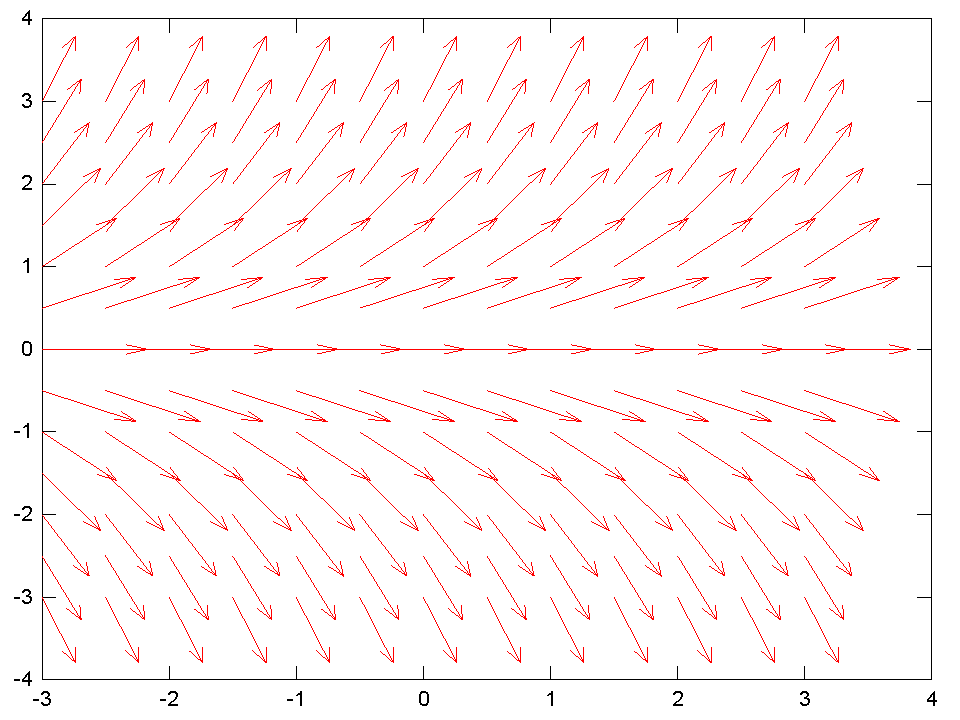
\includegraphics[width=0.48\textwidth]{trajektorien1.pdf}
	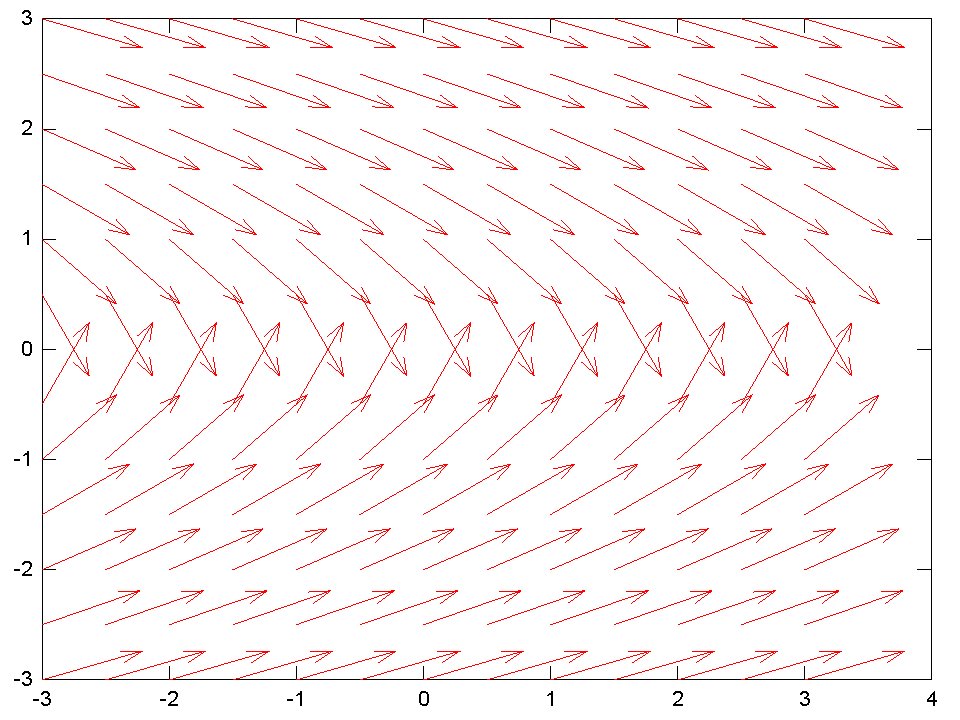
\includegraphics[width=0.48\textwidth]{trajektorien2.pdf}
	\caption{Ursprüngliche Kurvenschar (links, $y'=y$) 
	und orthogonale Trajektorie (rechts, $y'=-\frac{1}{y}$)}
\end{figure}

\newpage

\ifti
\subsection{Richtungsfeld plotten mit dem TI-89}
Um das Richtungsfeld mit dem TI-89 zu plotten, muss zuerst der Modus 
für Graphen auf Differentialgleichungen gesetzt werden. Danach kann die
gewünschte Differentialgleichung wie gewohnt definiert werden für das
Plotten. Wichitg ist zu beachten, dass der TI-89 hier Funktionen der Form 
$y(t)$ und nicht $y(x)$ verlangt!

\begin{enumerate}
	\item Modus für Graphen auf Differentialgleichungen setzen: \\
		\verb?HOME? 
		$\rightarrow$ \verb?Graph? 
		$\rightarrow$ \verb?DIFF EQUATIONS?
	\item Differentialgleichung Definieren: \\
		\verb?HOME?
		$\rightarrow$ $\diamond$
		$\rightarrow$ \verb?Y=?
		$\rightarrow$ DGL eingeben in \verb?y1'=? \\
		$\rightarrow$ falls gegeben den Anfangswert 
			$y'(0)=$ eingeben in \verb?yi1? 
	\item Graph plotten: \\
		\verb?HOME?
		$\rightarrow$ $\diamond$
		$\rightarrow$ \verb?GRAPH?
\end{enumerate}

\begin{figure}[h!]
	\centering
	% http://www.prenhall.com/esm/app/calc_v2/calculator/medialib/Technology/Documents/TI-89/desc_pages/slope_f.html
	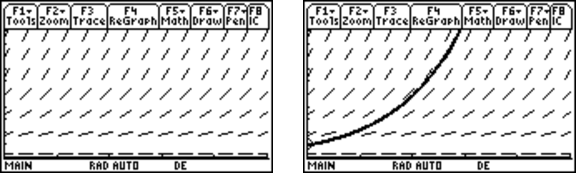
\includegraphics[scale=0.7]{ti89-plot-dgl.pdf}
	\caption{TI-89 Plot einer DGL ohne und mit Anfangswert.}
\end{figure}

\fi

\newpage
\section{Lösungsverfahren}

\subsection{Übersicht}
\begin{figure}[h!]
	\centering
	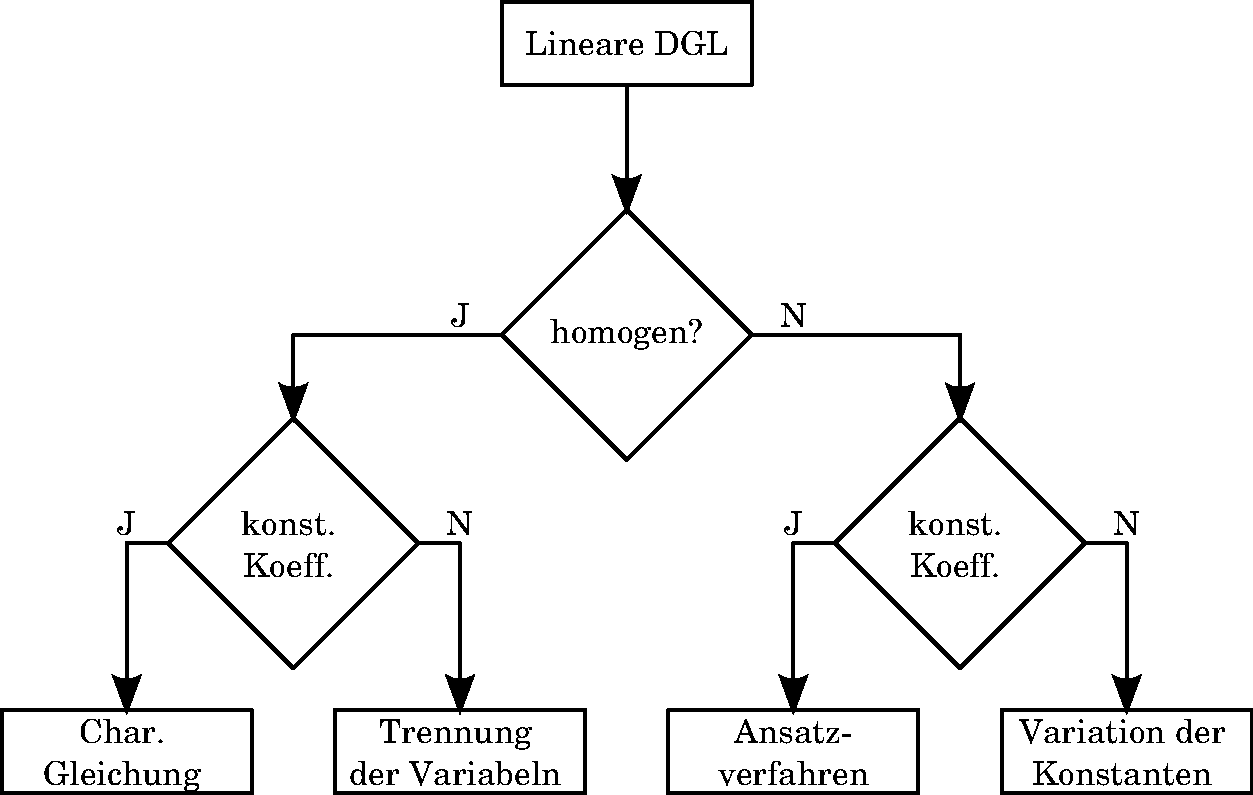
\includegraphics[width=1\textwidth]{diffgl_loes.pdf}
	\caption{Übersicht der Lösungsverfahren für Differentialgleichungen 
	erster Ordnung}
\end{figure}

\subsection{Variabelntrennung}
\begin{enumerate}
  \item $y'$ durch $\dfrac{dy}{dx}$ ersetzen
  \item alle $x$ und $y$ jeweils auf eine Seite bringen
  \item beide Seiten integrieren (Integrationskonstante nicht vergessen!)
  \item nach $y$ auflösen wenn möglich (sonst implizite Lösung)
\end{enumerate}

\subsection{Variation der Konstanten \\(Lineare Gleichung 1. Ordnung)}
\begin{enumerate}
  \item Inhomogene Gleichung notieren / aufstellen (I)
  \item Normalform bilden / aufstellen (N)
  \item Homogene Gleichung bilden / aufstellen (H)
  \item $g(x)$ und $G(x)$ bestimmen ($G(x) = \int g(x) ~ dx$) \\
        $g(x)$ ist der Koeffizient des Gliedes der nullten Ableitung. \\
        $x$ ist dabei die unabhängige Variable. 
  \item $G(x)$ einsetzen in die allgemeine Lösung $y_h=c \cdot e^{-G(x)}$
        $\rightarrow$ so erhält man die allgemeine Lösung der 
        homogenen Gleichung (H)
  \item Variation der Konstanten d.h. aus dem c wird eine Funktion $K(x)$ 
        $(\rightarrow y= \ldots)$
  \item Funktion ableiten (für $y'$)
  \item Die neuen Definitionen für $y$ und $y'$ einsetzen in die Normalform (N) 
  \item Auflösen nach $K(x)$ (durch Integration) \\
        Achtung! Integrationskonstante nicht vergessen! 
  \item Einsetzen in die allgemeine Lösung der homogenen Gleichung ($y_h$)
\end{enumerate}

\subsection{Charakteristische Gleichung}
Bei diesem Verfahren wird die Differentialgleichung in eine charakteristische 
Gleichung überführt. Dabei wird die abhängige Variable zu $k^{n}$ überführt. 
Der Exponent ($n$) von k entspricht dabei der Ordnung der Ableitung der 
unabhängigen Variable. 
\begin{enumerate}
  \item Homogene Gleichung aufstellen
  \item charakteristische Gleichung aufstellen
    \begin{itemize}
      \item $y \rightarrow k^0 = 1$
      \item $y' \rightarrow k^1 = k$
      \item $y'' \rightarrow k^2$
      \item $\cdots$
    \end{itemize}
  \item nach $k$ auflösen
  \item $k$ in die allgemeine Lösung der homogenen Gleichung einsetzen\\\\
        $\rightarrow y = c \cdot e^{k \cdot x}$
\end{enumerate}

\subsection{Ansatzverfahren}
Zur Bestimmung einer partikulären Lösung mit dem Ansatzverfahren wird die 
Störfunktion auf Funktionstypen analysiert. D.h. man versucht alle in der
Störfunktion enthaltenen Funktionstypen zu erkennen. Dies wird grundsätzlich
dadurch erreicht, indem man die Störfunktion ableitet, bis keine neuen 
Funktionstypen entstehen. Alternativ kann auch eine Tabelle benutzt werden.

\begin{enumerate}
	\item Inhomogene Gleichung aufstellen (I)
	\item Homogene Gleichung aufstellen (H)
	\item Charakteristische Gleichung aufstellen und nach k auflösen\\
		  $\Rightarrow$ allgemeine Lösung der homogenen Gleichung 
		  $y_h = c\cdot e^{k\cdot x}$
	\item Ansatz für die Störfunktion ermitteln \\
		  $\Rightarrow$ Partikuläre Lösung $y_p$ 
          \begin{itemize}
              \item Um den Ansatz zu ermitteln, wird die Störfunktion 
                    abgeleitet. 
              \item Die dabei auftretenden Funktionstypen werden dabei mit 
                    jeweils neuen Koeffizienten notiert. 
              \item Die Störfunktion wird so lange abgeleitet, bis keine neuen 
                    Funktionstypen mehr auftreten. 
              \item \textbf{Achtung!} Wenn ein Term dabei die homogene 
                    Gleichung löst, so muss dieser mit der unabhängigen 
                    Variable multipliziert werden. 
          \end{itemize}
	\item $y_p$ ableiten $\Rightarrow y_p'$
	\item $y_p$ und $y_p'$ in die inhomogene Gleichung einsetzen
		  und mit der Störfunktion gleichsetzen.
	\item Koeffizientenvergleich durchführen, Koeffizienten bestimmen.
	\item Koeffizienten einsetzen in die allgemeine Lösung $y=y_h + y_p$
	\item Falls gegeben, die Anfangsbedingungen einsetzen und restliche 
		  Koeffizienten ermitteln.
\end{enumerate}

\scriptsize
% Dieser Quelltext stammt von Peter Scheiblechner (C) 

\def\arraystretch{1.5}
\begin{tabular}{p{0.2\textwidth}|p{0.7\textwidth}}
%\begin{tabular}{ll}
\hline
St\"orfunktion $s(x)$ & Ansatz $y_p$ \\
\hline
$e^{\lambda x}$ & 
$
\left\{
\begin{array}{rl}
Ae^{\lambda x}, & \text{falls } s(x) \text{ keine L\"osung der homogenen Differentialgl.} \\
Axe^{\lambda x}, & \text{falls } s(x) \text{ L\"osung der homogenen Differentialgleichung}
\end{array} \right.
$ \\
$\sin \omega x$ & $A\sin \omega x+B\cos\omega x$ \\
$\cos \omega x$ & $A\sin \omega x+B\cos\omega x$ \\
$e^{\lambda x}\sin \omega x$ & $Ae^{\lambda x}\sin \omega x+Be^{\lambda x}\cos\omega x$ \\
$e^{\lambda x}\cos \omega x$ & $Ae^{\lambda x}\sin \omega x+Be^{\lambda x}\cos\omega x$ \\
$P_n(x)$ & $A_n x^n+A_{n-1} x^{n-1}+\cdots+A_1 x+A_0$ \\
$P_n(x)e^{\lambda x}$ & 
$
\left\{
\begin{array}{rl}
(A_n x^n+A_{n-1} x^{n-1}+\cdots+A_1 x+A_0)e^{\lambda x}, & \text{falls } e^{\lambda x} \text{ keine L\"osung} \\
 & \text{der homogenen DGL} \\
x(A_n x^n+A_{n-1} x^{n-1}+\cdots+A_1 x+A_0)e^{\lambda x}, & \text{falls } e^{\lambda x} \text{ L\"osung der} \\
 & \text{homogenen DGL} \\
\end{array} \right.
$ \\
$P_n(x)\sin \omega x$ & $(A_n x^n+A_{n-1} x^{n-1}+\cdots+A_1 x+A_0)\sin \omega x$ \\
 & \qquad$+(B_n x^n+B_{n-1} x^{n-1}+\cdots+B_1 x+B_0)\cos\omega x$ \\
$P_n(x)\cos \omega x$ & $(A_n x^n+A_{n-1} x^{n-1}+\cdots+A_1 x+A_0)\sin \omega x$ \\
 & \qquad$+(B_n x^n+B_{n-1} x^{n-1}+\cdots+B_1 x+B_0)\cos\omega x$ \\
$P_n(x)e^{\lambda x}\sin \omega x$ & $(A_n x^n+A_{n-1} x^{n-1}+\cdots+A_1 x+A_0)e^{\lambda x}\sin \omega x$ \\
 & \qquad$+(B_n x^n+B_{n-1} x^{n-1}+\cdots+B_1 x+B_0)e^{\lambda x}\cos\omega x$ \\
$P_n(x)e^{\lambda x}\cos \omega x$, & $(A_n x^n+A_{n-1} x^{n-1}+\cdots+A_1 x+A_0)e^{\lambda x}\sin \omega x$ \\
 $\omega\neq 0$ & \qquad$+(B_n x^n+B_{n-1} x^{n-1}+\cdots+B_1 x+B_0)e^{\lambda x}\cos\omega x$ \\
\end{tabular}

\normalsize

\newpage
\footnotesize
% coding:utf-8

% Quelle: Supersaxo Mario

\subsubsection*{Ansatztabelle nach Supersaxo}
\def\arraystretch{1.5}
\noindent
\begin{longtable}{@{}l|l|l}
\hline
Störfunktion $s(x)$ & $\gamma$ & Standardansatz \\
\hline
$x$ 
	& $0$ 
	& $ax+b$ \\
$\xi x$ 
	& $0$ 
	& $ax+b$ \\
$x^2$ 
	& $0$ 
	& $ax^2+bx+c$ \\
$\xi x^2$ 
	& $0$ 
	& $ax^2+bx+c$ \\
\vdots & \vdots & \vdots \\
$sin(\omega x)$
	& $\omega j$
	& $asin(\omega x)+bcos(\omega x) $ \\
$x sin(\omega x)$ 
	& $\omega j$ 
	& $(ax+b)sin(\omega x)+(cx+d)cos(\omega x)$ \\
$x^2 sin(\omega x)$ 
	& $\omega j$ 
	& $(ax^2+bx+c)sin(\omega x)+(dx^2ex+f)cos(\omega x)$ \\
\vdots & \vdots & \vdots \\
$x^{\xi}sin(\omega x)+x^{\psi}cos(\omega x)$, $\xi>\psi$
	& $\omega$ 
	& $P_{\xi}(x)sin(\omega x) + P_{\xi}cos(\omega x)$ \\
$x^{\xi}sin(\omega x)+x^{\psi}cos(\omega x)$, $\xi<\psi$
	& $\omega$ 
	& $P_{\psi}(x)sin(\omega x) + P_{\psi}cos(\omega x)$ \\
\vdots & \vdots & \vdots \\
$e^{\omega x}$ 
	& $\omega$ 
	& $ae^{\omega x}$ \\ 
$\xi e^{\omega x}$ 
	& $\omega$ 
	& $ae^{\omega x}$ \\ 
$x+e^{\omega x}$ $\rightarrow s_1(x),s_2(x)$ 
	& $0,\omega$ 
	& $s_1\rightarrow ax+b$, $s_2\rightarrow ce^{\omega x}$ \\
\vdots & \vdots & \vdots \\
$x e^{\omega x}$ 
	& $\omega$ 
	& $(ax+b)e^{\omega x}$ \\
$(\xi+x)e^{\omega x}$ 
	& $\omega$ 
	& $(ax+b)e^{\omega x}$ \\
$xe^{\omega x}+\xi e^{\psi x} \rightarrow s_1(x), s_2(x)$ 
	& $\omega,\xi$ 
	& $s_1\rightarrow (ax+b)e^{\omega}, s_2\rightarrow ae^{\psi x}$ \\
\end{longtable}

\noindent
\textbf{Achtung:} Bei $e$-Funktionen muss überprüft werden ob der gewählte Ansatz 
eine Lösung der homogenen Gleichung darstellt. Falls dies zutrifft, muss der
Ansatz mit der unabängigen Variable erweitert werden. Dies wiederholt 
man so lange, bis es nicht mehr eine Lösung der homogenen Gleichung darstellt.

\normalsize

\newpage

\section{Lineare DGL zweiter Ordnung}
Spricht man von linearen Differentialgleichungen zweiter Ordnung, 
so heisst dies, dass die abhängige Variable zweifach abgeleitet
vorkommt.
\[ a\cdot y'' + b \cdot y' + c \cdot y = \tilde{s}(x) 
   \qquad \text{allgemeine Form}\]
\[ y'' + a_1 \cdot y' + a_0 \cdot y = s(x) 
   \qquad \text{Normalform}\]
   \[  s(x) \neq 0 \qquad \text{Inhomogen} \]
   \[  s(x) =    0 \qquad \text{Homogen} \]

\subsection{Homogene Gleichung}
Zwei Funktionen $y_1(x)$ und $y_2(x)$ heissen linear abhängig falls
\[ y_1(x)=c \cdot y_2(x) \qquad \text{oder} \qquad y_2(x)=c \cdot y_1(x) \]
wobei $c$ eine Konstante ist. Anderenfalls heissen $y_1(x)$ und $y_2(x)$
linear unabhängig.

\subsubsection{Satz}
\begin{itemize}
  \item Sind $y_1(x)$ und $y_2(x)$ Lösungen der homogenen Gleichung,
	so ist die neue Funktion 
	\[ y(x) = c_1y_1(x) + c_2y_2(x) \]
	wieder eine Lösung der homogenen Gleichung, wobei $c_1, c_2$
	beliebige Konstanten sind.
  \item Sind $y_1(x)$ und $y_2(x)$ linear unabhängige Lösungen der 
	homogenen Gleichung, so ist
	\[ y=c_1y_1 + c_2y_2 \qquad c_1, c_2 \in \mathbb{R} \]
	die allgemeine Lösung der homogenen Gleichung.
\end{itemize}

\subsubsection{Lösungsverfahren}
Um eine lineare homogene Differentialgleichung zweiter Ordnung zu 
lösen, kann wie folgt vorgegangen werden.
\begin{enumerate}
  \item Inhomogene Gleichung aufstellen
  \item Normalform bilden
  \item Homogene Gleichung sinngemäss notieren
	\[ y'' + a_1y' + a_0y = 0 \]
  \item Charakteristische Gleichung aufstellen.\\
	Der Ansatz hierzu: $y=e^{kx}$ somit ist $y'=k\cdot e^{kx}$
	und $y''=k^2 \cdot e^{kx}$.
	\[ k^2 + a_1k + a_0 = 0 \]
  \item Gleichung nach $k$ auflösen mit der Formel
	\[ k_{1,2} = \frac{1}{2}\left(-a_1 \pm \sqrt{{a_1}^2 - 4 \cdot a_0}\right) \]
\item Diskriminante $({a_1}^2 - 4 \cdot a_0)$ betrachten und entsprechend einsetzten
	\begin{itemize}
	  \item $D > 0$ zeigt zwei reelle Lösungen an\\
		\[ y=c_1e^{k_1x} + c_2e^{k_2x} \]
          \item $D = 0$ zeigt zwei gleiche reelle Lösungen an\\
		\[ y=c_1e^{kx} + c_2xe^{kx} \]
          \item $D < 0$ zeigt zwei komplexe Lösungen an\\
		\[ k=\mu \pm j \omega \]
		\[ y=c_1e^{\mu x} cos(\omega x) + c_2e^{\mu x} sin(\omega x) \]
		Wie es zu einer komplexen Lösung kommt: 
		Wenn die Diskriminate $D < 0$ ist, so kann der Wurzelausdruck
		statt z.B. $\sqrt{-25}$ als 
		$\sqrt{(-1)25}=\sqrt{-1}\sqrt{25}=\pm j5$ geschrieben werden.
		Dies wäre dann das $j\omega$ aus obiger Formel.
	\end{itemize}
\end{enumerate}

\subsection{Inhomogene Gleichung}

\subsubsection{Lösungsverfahren}
Bei einer inhomogenen Gleichung mit konstanten Koeffizienten kann das 
Ansatzverfahren angewendet werden. 
\begin{enumerate}
  \item Inhomogene Gleichung aufstellen
  \item Normalform bilden
  \item Homogene Gleichung sinngemäss notieren
	\[ y'' + a_1y' + a_0y = 0 \]
  \item Charakteristische Gleichung aufstellen.\\
	Der Ansatz hierzu: $y=e^{kx}$ somit ist $y'=k\cdot e^{kx}$
	und $y''=k^2 \cdot e^{kx}$.
	\[ k^2 + a_1k + a_0 = 0 \]
  \item Gleichung nach $k$ auflösen mit der Formel
	\[ k_{1,2} = \frac{1}{2}\left( -a_1 \pm \sqrt{a_1^2 - 4a_0} \right)  \]
  \item Diskriminante betrachten und entsprechend einsetzten
	\begin{itemize}
	  \item $D > 0$ zeigt zwei reelle Lösungen an\\
		\[ y_h=c_1e^{k_1x} + c_2e^{k_2x} \]
          \item $D = 0$ zeigt zwei gleiche reelle Lösungen an\\
		\[ y_h=c_1e^{kx} + c_2xe^{kx} \]
          \item $D < 0$ zeigt zwei komplexe Lösungen an\\
		\[ k=\mu \pm j \omega \]
		\[ y_h=c_1e^{\mu x} cos(\omega x) + c_2e^{\mu x} sin(\omega x) \]
		Wie es zu einer komplexen Lösung kommt: 
		Wenn die Diskriminate $D < 0$ ist, so kann der Wurzelausdruck
		statt z.B. $\sqrt{-25}$ als 
		$\sqrt{(-1)25}=\sqrt{-1}\sqrt{25}=\pm j5$ geschrieben werden.
		Dies wäre dann das $j\omega$ aus obiger Formel.
	\end{itemize}
  \item Ansatz für die Störfunktion ermitteln per Tabelle oder von Hand: \\
    $\Rightarrow$ Partikuläre Lösung $y_p$ 
    \begin{itemize}
      \item Um den Ansatz zu ermitteln, wird die Störfunktion 
            abgeleitet. 
      \item Die dabei auftretenden Funktionstypen werden dabei mit 
            jeweils neuen Koeffizienten notiert. 
      \item Die Störfunktion wird so lange abgeleitet, bis keine neuen 
            Funktionstypen mehr auftreten. 
      \item \textbf{Achtung!} Wenn ein Term dabei die homogene 
            Gleichung löst, so muss dieser mit der unabhängigen 
            Variable multipliziert werden. 
    \end{itemize}
  \item $y_p$ so oft ableiten wie die Ordnung der Gleichung 
        $\Rightarrow y_p', y_p'', \ldots$
  \item $y_p$, $y_p'$, $\ldots$ in die inhomogene Gleichung einsetzen
        und mit der Störfunktion gleichsetzen.
  \item Koeffizientenvergleich durchführen, Koeffizienten bestimmen.
  \item Koeffizienten einsetzen in die allgemeine Lösung $y=y_h + y_p$
  \item Fall gegeben, die Anfangsbedingungen einsetzen und restliche 
        Koeffizienten ermitteln. 
\end{enumerate}

\ifti
\section{Diffentialgleichungen mit TI-89 lösen}
\verb?deSolve(EQUATION, INDEP-VAR, DEPEND-VAR)? \\\\
\begin{tabular}{@{}ll}
	\verb?EQUATION?
		& Differentialgleichung (und Bedingungen) \\
	\verb?INDEP-VAR?
		& unabhängige Variable \\
	\verb?DEPEND-VAR?
		& abhängige Variable \\
\end{tabular}\\\\
Bsp.: Man möchte die Differentialgleichung $y'(x)=-y(x)-x$ lösen.
Über die Taste \verb?CATALOG? gelangt man in die Auswahl, tippt \verb?d?
an für \textit{deSolve} und wählt es per \verb?ENTER? aus.
Danach gibt man die verlangten Angaben an:\\\\
\indent
\verb?deSolve(y'=-y+2*x,x,y)?\\\\ 
erzeugt die Ausgabe \\\\
\indent
\verb?y=@47*e^(-x)+2*(x-1)? \\\\
Der Faktor, welcher mit \verb?@? angezeigt wird, stellt die 
Integrationskonstante dar, d.h. das vorherige \verb?@47? ist einfach $c$.
Man kann aber auch gleich die Bedingung zur Differentialgleichung 
hinzufügen (z.B. $y(0)=0$ oder $y(1)=3$) mittels eines \verb?and?.
Somit liefert die Eingabe \\\\
\indent
\verb?deSolve(y'=-y+2*x and y(0)=0,x,y)? \\\\
das Ergebnis \\\\
\indent
\verb?y=2*((x-1)*e^(x)+1)*e^(-x)?\\\\
Wichtig ist zu beachten, dass der TI-89 nur Differentialgleichungen
von erster und zweiter Ordnung analytisch lösen kann!
\fi
